\chapter{Interactive Perception Library}
\label{chapter:Interactive Perception Library}


\section{Motivation and Goals}
%Since we understand the world based on functionality and behavior, as a result, manipulation becomes an integral part of perception. In other words, purposeful manipulation depends on the robot's ability to curiously explore its unknown environment through interaction. 

Based on the increasing popularity of the interactive perception approach, we created a common place that unites researchers' efforts towards better algorithms and systems that concern adding manipulation in the perception loop. In addition, we developed a generic framework which can be of great help for sharing different implementations of similar problems. So far, we have received positive feedback from various institutions that decided to join the initiative, among others: Robotic Institute at Carnegie Mellon University, Robotics and Biology Laboratory at Technical University Berlin, Robotics Group at Robert Bosch LLC, Robotic Intelligence Laboratory at Universitat Jaume I. Having seen the success achieved by similar initiatives (e.g. openslam.org, OpenCV, PCL, etc.) in other fields, we want to follow in their footsteps in order to create a synergistic community of interactive perception researchers.

It is worth emphasising and it has been shown in Chapter \ref{chapter:Related Work}, that interactive perception field has gained many more potential applications than the ones presented in this thesis. These applications include interactive perception methods for object segmentation, modelling, grasping, and learning manipulation skills through interactive perception. Interestingly, these results begin to appear independently in the different relevant communities: perception, manipulation, and learning.

Keeping this in mind, we created a common, modular tool - Interactive Perception Library\footnote{\url{http://github.com/Lolu28/interactive_perception}}, which addresses researchers' needs to investigate interactive perception area more deeply and enables easier access to existing resources and algorithms. The main goal of this library is to collect all the code from different laboratories involved in the field of interactive perception. We developed a framework that enables users to switch between different implementations of each module from the interactive perception pipeline at runtime. We implemented everything in ROS since it is easier to support various robots, include datasets, and glue different algorithms together. 


\section{Library}
\subsection{Modules}
Looking at various systems created by different robotics institutes \todo{: REF} it can be noticed that there is a similar idea lying behind them. After conducting research in existing implementations, we noticed many similar modules that became crucial for our library, those being:

\begin{itemize}
\item Static Segmentation - performs static segmentation in the scene and infers which parts of the scene are most likely to be segmented incorrectly
\item Feature Extraction - extracts features that will be tracked
\item Push Point Estimation - finds the best point to interact with objects
\item Manipulation - manipulates a robot's arm in order to interact with objects in the scene
\item Tracking - tracks previously extracted features during a robot's movement
\item Trajectory Clustering - clusters the trajectories of the features that have moved in the same manner
\item Full Reconstruction - reconstructs a full model of the object. It takes the sparse representation (clustered features) and reconstructs a dense model of the object.
\end{itemize}

Since the interactive perception systems use a model-based approach, we incorporated feature extraction module. In order to improve robustness of algorithms, we included the static segmentation module which works as a pre-processing step for our system. Having in mind potential applications such as grasping and object recognition, we included a dense model reconstruction module.

The library was created based on the abstract factory pattern and it mainly uses pluginlib\footnote{\url{http://ros.org/wiki/pluginlib}} from ROS. The main executable shows a simple user interface together with a visualization tool (ROS package - \textit{Visualizer}). The user interface shows a possibility to call different modules and their particular implementations by using a simple GUI - \textit{dynamic reconfigure} ROS package\footnote{\url{http://www.ros.org/wiki/dynamic_reconfigure}}. The details are described in the next section.

\subsection{Architecture}

In order to describe the architecture, it is needed to explain the idea of the pluginlib library that was heavily used in this project. Pluginlib is a C++ library that enables users to load and unload other classes (plugins) dynamically without being explicitly linked against their implementations. In this way, pluginlib can open a library that it was not aware of before running the program. 

This tool gives us a number of possibilities that can be used in the Interactive Perception Library. Keeping in mind all the modules that we depicted in the previous sections, we can dynamically switch between different implementations of each of these modules. For example, if we want to combine two different interactive perception algorithms, we can simply mix the modules from their pipelines by dynamically loading them. 

In addition, the library contains graphical debug tools that enable users to visualize the currently loaded point cloud as depicted in Figure \ref{fig:ipl}. It also provides the functionality of visualizing different outputs such as customized point types and point normals.

\begin{figure}
%\centering

{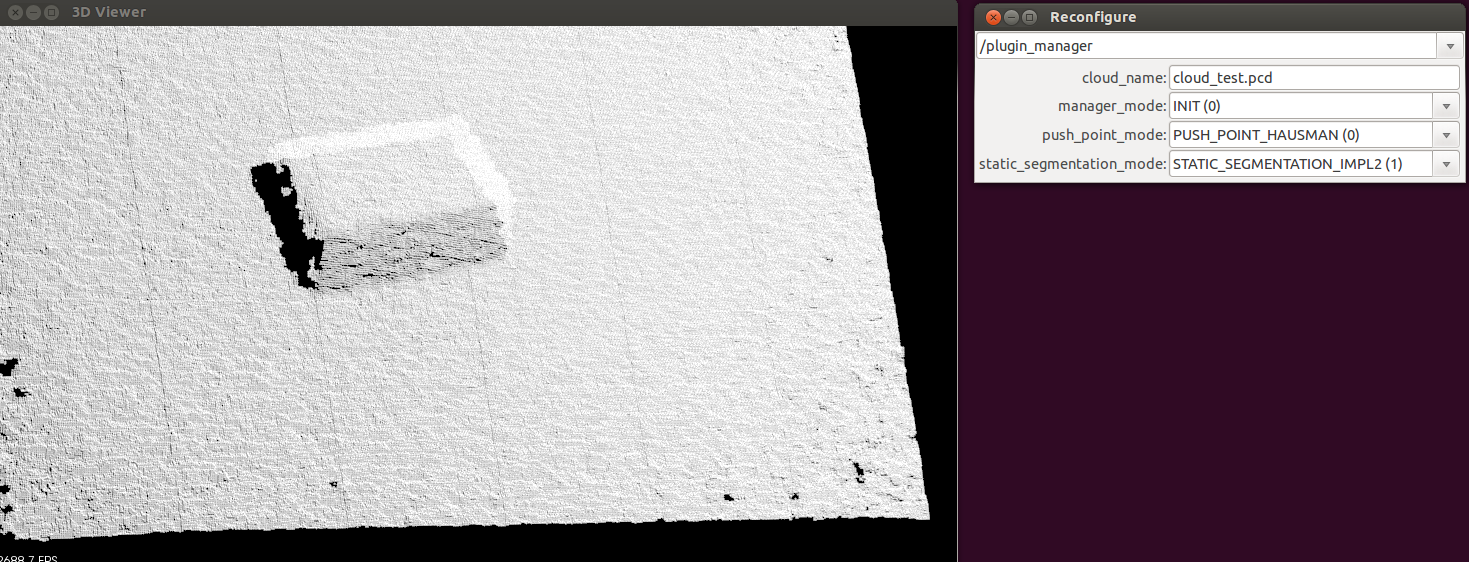
\includegraphics[width=1.1\columnwidth]{figures/ipl.png}}

\caption{Interactive Perception Library with running \textit{visualizer} and a simple Graphical User Interface to choose the module and its implementation.}
\label{fig:ipl}
\end{figure}

The architecture is presented in Figure \ref{fig:uml}, in the form of an UML class diagram. There is a main class called \textit{PluginManager} that is responsible for loading different plugins and executing respective steps of the algorithm. It delegates the visualization tasks to the class named \textit{Visualizer}. The only connection that \textit{PluginManager} has to the plugins is through the \textit{interactive perception interface} ROS package that consists of all the interfaces for different modules. In addition to that, there are ROS packages holding an implementation of the respective module. In Figure \ref{fig:uml} there are two different implementations for two interfaces - \textit{StaticSegmentation} and \textit{PushPointEstimation}. The user can dynamically switch between \textit{PushPointImpl} and \textit{PushPointImpl2} since both of them implement the same generic interface. This design enables other people to benchmark their modules against other algorithms and also to find the combination that best fits their application.  

\begin{figure}
%\centering
{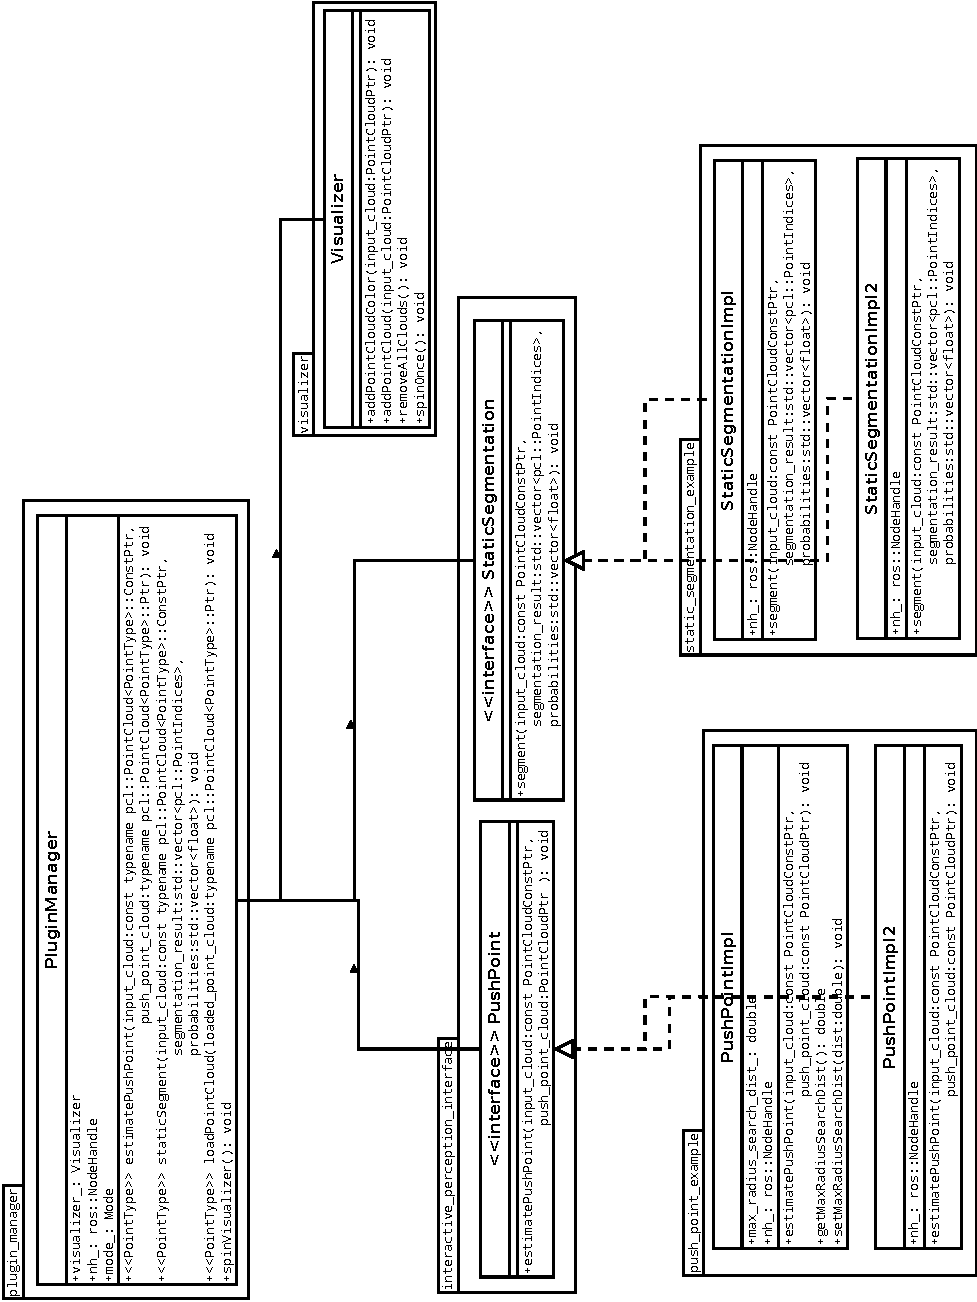
\includegraphics[width=0.9\columnwidth, angle=-90]{figures/uml-after.pdf}}

\caption{UML class diagram that shows the main structure of the library.}
\label{fig:uml}
\end{figure}




